\documentclass{beamer}
\usepackage{listings}
\usepackage{verbatim}
\usepackage{hyperref}

\usetheme{progressbar}
\progressbaroptions{titlepage=normal, frametitle=normal}

\title{Android RIL - Radio Interface Layer}
\institute{Elektrobit Wireless(2011)}
\author{Lifu Zhang}
\date{}
\logo{
\includegraphics[width=1cm]{linuxfb-logo.png}}

\definecolor{codeBg}{HTML}{EFFFD0}
\begin{document}
\setbeamertemplate{background}{
\includegraphics[height=\paperheight]{progressbar/slide.png}}
%\newcommand{\scriptsize}{\fontsize{14pt}{12pt}\selectfont}
\lstset{% general command to set parameter(s)
basicstyle=\fontsize{6pt}{6pt}\ttfamily,
% print whole listing small
keywordstyle=\color{blue}\bfseries,
% underlined bold black keywords
identifierstyle=\color{black},
% nothing happens
stringstyle=\color{red}\ttfamily,
% typewriter type for strings
showstringspaces=false,
breaklines=true,
% no special string spaces
backgroundcolor=\color{codeBg}
}

\maketitle

\section*{Outline}
\begin{frame}
  \frametitle{Outline}
  \tableofcontents
\end{frame}

\section{Android Telephony}
\begin{frame}
    \frametitle{Terms}
    \begin{itemize}
        \item RIL Daemon: The RIL daemon initializes the Vendor RIL, processes all communication from Android telephony services, and dispatches calls to the Vendor RIL as solicited commands. 
        \item Vendor RIL: The radio-specific Vendor RIL of ril.h that processes all communication with radio hardware and dispatches calls to the RIL Daemon (rild) through unsolicited commands.
    \end{itemize}
\end{frame}

\begin{frame}
    \frametitle{Architechture of Android Telephony}
    The telephony is based on these items, layout layer by layer \\
    \begin{itemize}
        \item Android Services, activities, call settings
            \begin{itemize}
                \item Service ``isms''
                \item Dialer application
                \item Other Telephony settings and operations
            \end{itemize}
        \item The com.android.internal.phone interface
        \item PhoneFactory, PhoneProxy, CDMAPhone, GSMPhone
        \item RIL.java
        \item ril-daemon
        \item vender ril
    \end{itemize}
\end{frame}

\subsection{Big Picture}
\begin{frame}
	\begin{columns}[c]
        \column{0.5in}
        Arch
        \column{3in}
        \framebox{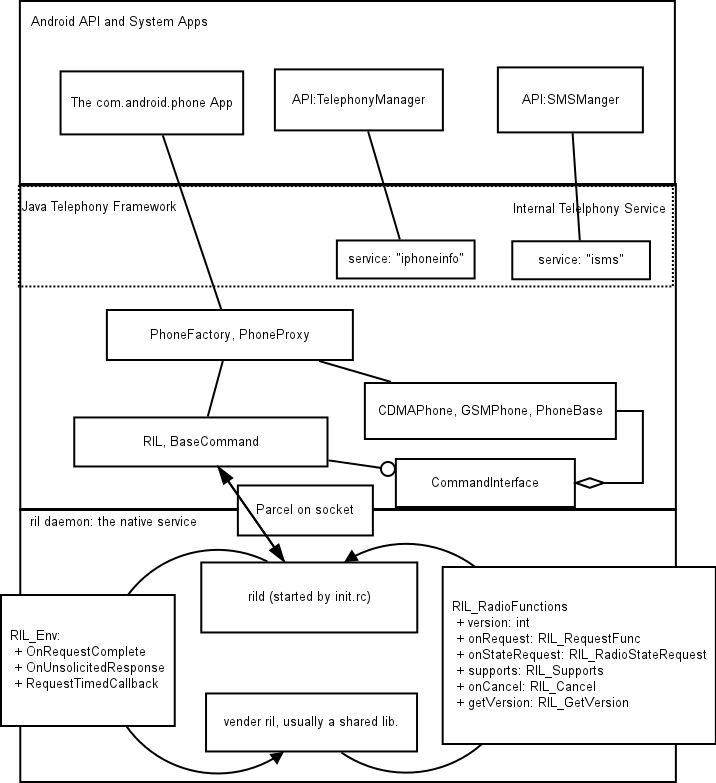
\includegraphics[width=3in]{ril/arch}}
    \end{columns}
\end{frame}

\begin{frame}
    \frametitle{Files in System}
    \begin{columns}[c]
        \column{2.25in}
            Source:
            \begin{itemize}
                \item com.android.telephony
                \item com.android.internal.telephony
                \item com.android.phone
                \item hardware/ril
            \end{itemize}
            
        \column{2.25in}
        Binary:
        \begin{itemize}
            \item /system/framework/ framework.jar
            \item /system/bin/rild
            \item /system/lib/libril.so
            \item /system/lib/lib(vender)-ril.so
        \end{itemize}
    \end{columns}
\end{frame}

\subsection{Porting Work}
\begin{frame}
    \frametitle{Our Job: libxxx-ril.so vender ril}
    \begin{itemize}
        \item The C Programming Language
        \item Control the modem, by whatever means (using tty now)
        \item Translate requests and data between framework and modem
    \end{itemize}
\end{frame}

\begin{frame}
	\begin{columns}[c]
        \column{0.5in}
        Our Job
        \column{3in}
        \framebox{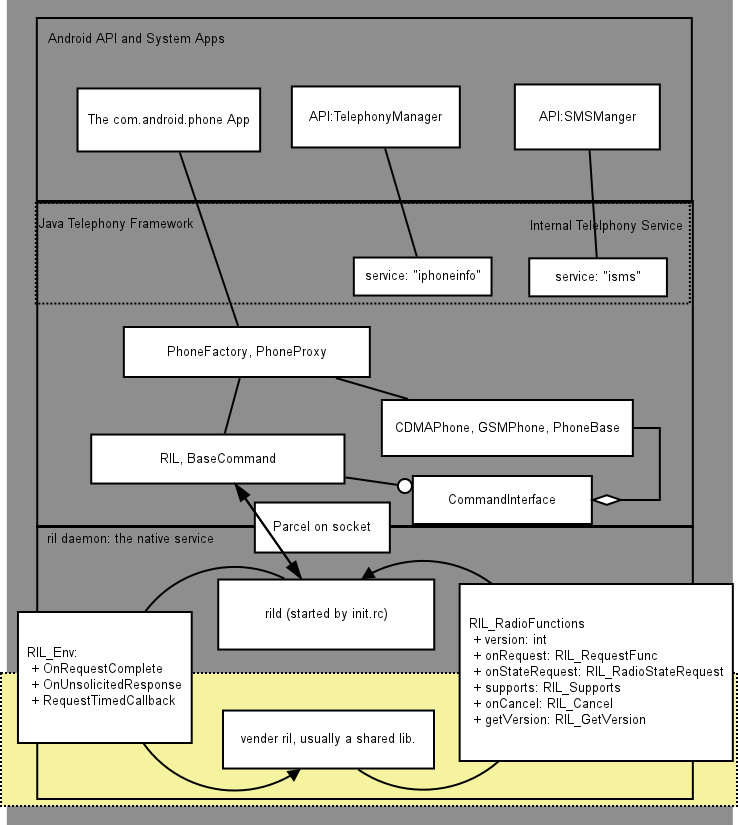
\includegraphics[width=3in]{ril/ourjob}}
    \end{columns}
\end{frame}

\subsection{Interacton between Framework and Local Service}

\begin{frame}
    \frametitle{Requests and Response - Async IPC}
    \begin{columns}[c]
        \column{2in}
        \begin{itemize}
            \item They are async, you don't have to response it immediately.
            \item All requests and response is handled by the RIL.java, then dispatched to upper framework
            \item The ril daemon will use some C++ code disamble the Parcel, and pass void * data to vender ril
        \end{itemize}
        \column{2in}
        \framebox{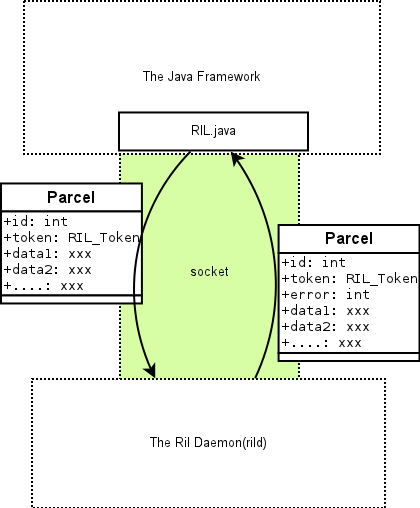
\includegraphics[height=2.4in]{ril/reqandresp}}
    \end{columns}
\end{frame}
 
\begin{frame}
    \frametitle{The Requests}
    \begin{itemize}
        \item requests is comming from the framework, packed as Parcel, trasfered on local socket, dispatched by rild, and handled by vender ril.
        \item request id: What do you want to do
        \item request token: just a token, using when response it
        \item request data: e.g. when sending sms, you have to specify address, text in the data
    \end{itemize}
\end{frame}

\begin{frame}
    \frametitle{The Response}
    \begin{itemize}
        \item the response is generated by vender ril, packed as Parcel, transfered on local socket, dispatched by CommandInterface, and handled by those who register its handler.
        \item id: same as the requests id
        \item error id: success or something wrong
        \item data: data is in format specify by the request, and if no data needed, it would be 'NULL'
        \item special: Some response is not to a request, we call they unsolicited responses.
    \end{itemize}
\end{frame}

\subsection {Ril Initilize}

\begin{frame}
    \frametitle{Ril initial sequence}
    \framebox{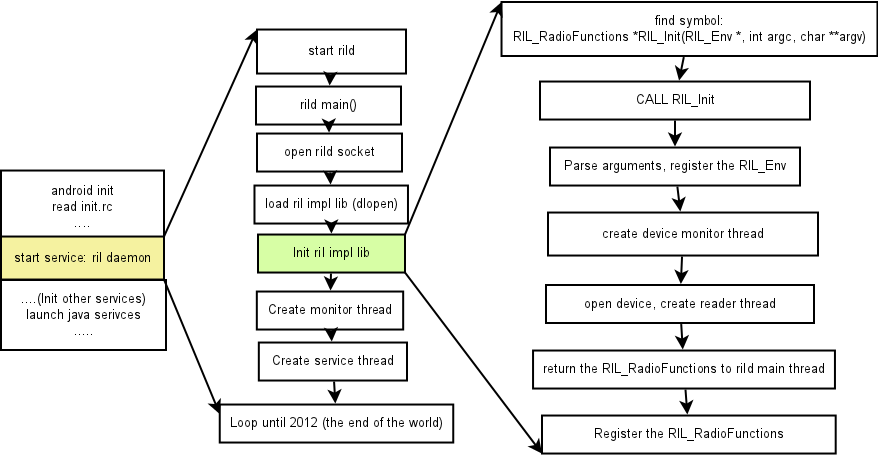
\includegraphics[height=2.4in]{ril/rilinit}}
\end{frame}

\begin{frame}[fragile]
    \frametitle{Init Code I - Load RIL Library}
    \lstset{language=C}
  \begin{lstlisting}

    dlHandle = dlopen(rilLibPath, RTLD_NOW);

    if (dlHandle == NULL) {
        fprintf(stderr, "dlopen failed: %s\n", dlerror());
        exit(-1);
    }

    RIL_startEventLoop();

    rilInit = (const RIL_RadioFunctions *(*)(const struct RIL_Env *, int, char **))
              dlsym(dlHandle, "RIL_Init");

    if (rilInit == NULL) {
        fprintf(stderr, "RIL_Init not defined or exported in %s\n", rilLibPath);
        exit(-1);
    }

 //.. omitted code .. 
    funcs = rilInit(&s_rilEnv, argc, rilArgv);

    RIL_register(funcs);

done:

    while(1) {
        // sleep(UINT32_MAX) seems to return immediately on bionic
        sleep(0x00ffffff);
    }
  \end{lstlisting}
\end{frame}

\begin{frame}[fragile]
    \frametitle{Init Code II - Wait for device ready}
    \lstset{language=C}
  \begin{lstlisting}
for (;;) {
    fd = -1;
    while  (fd < 0) {
        if (s_port > 0) {
            fd = socket_loopback_client(s_port, SOCK_STREAM);
        } else if (s_device_socket) {
            if (!strcmp(s_device_path, "/dev/socket/qemud")) {
                /*..CODE OMITTED.. Qemu-specific control socket */
            }
            else
                fd = socket_local_client( s_device_path,
                                        ANDROID_SOCKET_NAMESPACE_FILESYSTEM,
                                        SOCK_STREAM );
        } else if (s_device_path != NULL) {
            fd = open (s_device_path, O_RDWR);
            if ( fd >= 0 && isSerialPortDevice(s_device_path) ) { 
                /* set serial port acting in raw mode, CODE OMITTED .. */
                tcsetattr( fd, TCSANOW, &ios );
            }
        }
        if (fd < 0) {
            sleep(10);
        }
    }

    s_closed = 0;
    ret = at_open(fd, onUnsolicited);
    RIL_requestTimedCallback(initializeCallback, NULL, &TIMEVAL_0);
    // Give initializeCallback a chance to dispatched, since
    // we don't presently have a cancellation mechanism
    sleep(1);
    waitForClose();
}
  \end{lstlisting}
\end{frame}

\section{Vender RIL}
\begin{frame}
    \frametitle{The Vender RIL}
    In this sections, we'll have some examples about how the vender ril works.
    \begin{itemize}
        \item The Vender RIL and RIL Daemon is interact with RIL\_RadioFunctions and RIL\_Env facility.
        \item The Vender RIL is the very part of system that handle radio operations.
    \end{itemize}
\end{frame}

\begin{frame}[fragile]
    \frametitle{The RIL Enviroment and RIL Radio Functions}
     \lstset{language=C}
  \begin{lstlisting}
typedef void (*RIL_RequestFunc) (int request, void *data,
                                    size_t datalen, RIL_Token t);
typedef RIL_RadioState (*RIL_RadioStateRequest)();
typedef int (*RIL_Supports)(int requestCode);
typedef void (*RIL_Cancel)(RIL_Token t);
typedef void (*RIL_TimedCallback) (void *param);
typedef const char * (*RIL_GetVersion) (void);

typedef struct {
    int version;        
    RIL_RequestFunc onRequest;
    RIL_RadioStateRequest onStateRequest;
    RIL_Supports supports;
    RIL_Cancel onCancel;
    RIL_GetVersion getVersion;
} RIL_RadioFunctions;
  \end{lstlisting}
     \lstset{language=C}
  \begin{lstlisting}
struct RIL_Env {
    void (*OnRequestComplete)(RIL_Token t, RIL_Errno e,
          void *response, size_t responselen);
    void (*OnUnsolicitedResponse)(int unsolResponse,
          const void *data,
          size_t datalen);
    void (*RequestTimedCallback) (RIL_TimedCallback callback,
          void *param, 
          const struct timeval *relativeTime);
};
  \end{lstlisting}
\end{frame}
\begin{frame}
    \frametitle{NOTES}
    \begin{itemize}
        \item functions in RIL\_Env is used by vender ril, and RIL\_RadioFunctions is used by rild
        \item The vender rilementation is in the same process space as ril-daemon
        \item onComplete is re-enterable, (will block by a mutex if called by multi-thread in same time)
    \end{itemize}
\end{frame}

\begin{frame}
    \frametitle{Operation to the modem}
    \framebox{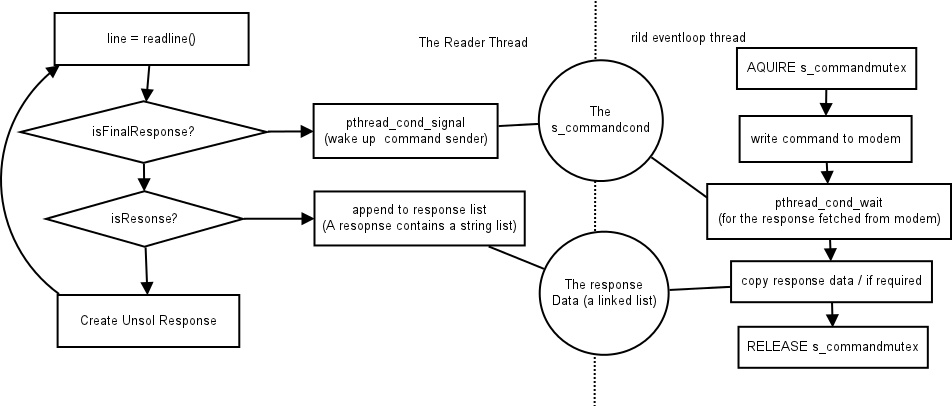
\includegraphics[width=4.5in]{ril/modemop}}
\end{frame}

\begin{frame}
    \frametitle{Summary: Threads in rild process space}
    \begin{itemize}
        \item rild main thread: parse argc, argv, open ril library, create event loop, some timed call back is run in this thread.
        \item rild event loop: handle requests from upper layer, and call OnRequests of vender ril.
        \item vender reader loop: read data comming from modem, packed as response/unsol response.
    \end{itemize}
\end{frame}

\subsection {Example I: Signal Strength}
\begin{frame}
    \frametitle{Example I: Signal Strength Query/Report}
    The framework may query current signal strength(case I), and when modem detect a signal change, ril should report this event(case II).\\
    \begin{columns}[c]
        \column{2.5in}
        For Case I:
        \begin{itemize}
            \item Send 'AT+CSQ' command
            \item Waiting for response
            \item Parse response, pack data into RIL\_CDMA\_SignalStrength
            \item OnRequestComplete
        \end{itemize}
        \column{2in}
        For Case II:
        \begin{itemize}
            \item The reader loop recieve '+CSQxxxx'
            \item Parse the at command string pack data into RIL\_CDMA\_SignalStrength
            \item OnUnsolicitedResponse
        \end{itemize}
    \end{columns}
\end{frame}

\begin{frame}[fragile]
    \frametitle{Example I: Signal Strength Report - Code}
    \lstset{language=C}
  \begin{lstlisting}
static void onUnsolicited (const char *s, const char *sms_pdu)
{
//this is the function called when readerloop found an unsol modem command
//.. omitted code ..
    } else if (strStartsWith(s, "^HRSSILVL:")) {
        //handle signals here
        onHrssiChanged (s) ;
    }
 //.. omitted code ..
}
  \end{lstlisting}
  \begin{lstlisting}
static void onHrssiChanged(const char *s) 
{
    int sigStrength;
    int err;
    char *membak = strdup(s);
    char *ln = membak;
    RIL_SignalStrength sigsth;
    RIL_SignalStrength *sth = &sigsth;

    err = at_tok_start(&ln);
    if (err) goto error;
    err = at_tok_nextint(&ln, &sigStrength);
    if (err) goto error;

    hw_convertSignalStrengh (sigStrength, sth); //will do data convertion
    RIL_onUnsolicitedResponse (RIL_UNSOL_SIGNAL_STRENGTH, sth, sizeof(*sth) );

    free (membak);
    return;

error:
    free (membak);
    LOGE ("Unsol Signal Strength command error: %s", s);
    return;
}
  \end{lstlisting}
\end{frame}

\begin{frame}[fragile]
    \frametitle{Example I: Signal Strength Query - Code}
    \begin{columns}[c]
        \column{1in}
        \begin{itemize}
            \item SS query
            \item For Huawei modem
            \item with adaptation
        \end{itemize}

        \column{3.5in}
    \lstset{language=C}
  \begin{lstlisting}
    RIL_SignalStrength sth;
    int err = hw_getSignalStrength(&sth);

    if (! err) {
        RIL_onRequestComplete(t, RIL_E_SUCCESS, &sth, sizeof(sth));
    } else {
        RIL_onRequestComplete(t, RIL_E_GENERIC_FAILURE, NULL, 0);
    }

  \end{lstlisting}
    \lstset{language=C}
  \begin{lstlisting}
int hw_getSignalStrength (RIL_SignalStrength *sth)
{
    int err = 0;
    ATResponse *p_response;

    err = at_send_command_singleline ("AT^HDRCSQ", "^HDRCSQ", &p_response);
    char *line = p_response->p_intermediates->line;
    do {
        int hwhdr;
        if (err < 0 || p_response->success == 0) break;
        err = at_tok_start(&line);
        if (err) break;
        err = at_tok_nextint(&line, &hwhdr);
        if (err) break;
        hw_convertSignalStrengh(hwhdr, sth);
    }while (0);

    at_response_free(p_response);
    return err;
}
  \end{lstlisting}

    \end{columns}
\end{frame}

\subsection {Example II: Voice Call}
\begin{frame}
    \frametitle{Dial a Number}
    When the java framework wanna dial a number, it will send a request to rild:
    \begin{itemize}
        \item ID  : RIL\_REQUEST\_DIAL (value=10, int)
        \item Data: RIL\_Dial :\{
            \begin{itemize}
                \item address: char *, the address we'll dialing, e.g. 13xxxxxxxx
                \item clir: int, loop TS27.007 7.7 +CLIR, I don't know what's this.
                \item  uusInfo: RIL\_UUS\_Info *, NULL or Pointer to User-User Signaling Information
            \end{itemize}
            \}
    \end{itemize}
\end{frame}

\begin{frame}[fragile]
    \frametitle{What Shall I Do? Make the Call!}
    \lstset{language=C}
  \begin{lstlisting}
    p_dial = (RIL_Dial *)data;
    switch (p_dial->clir) {
        case 1: clir = "I"; break;  /*invocation*/
        case 2: clir = "i"; break;  /*suppression*/
        default:
        case 0: clir = ""; break;   /*subscription default*/
    }
    ret = sendDialCommand (p_dial->address, clir);
    RIL_onRequestComplete(t, (RIL_Errno)ret, NULL, 0);
  \end{lstlisting}
    \lstset{language=C}
  \begin{lstlisting}
static int sendDialCommand(const char *number, const char *clir)
{
    int ret;
    if (isInCall()) { //forbide call in call operation
        ret = RIL_E_GENERIC_FAILURE;
    } else { /*Not in call, us AT+CDV*/
        char *cmd;
        asprintf(&cmd, "AT+CDV%s%s;", number, clir);
        ret = at_send_command(cmd, NULL);
        free(cmd);
    }
    if (ret) {
        return RIL_E_GENERIC_FAILURE;
    } else {
        return RIL_E_SUCCESS;
    }
}
  \end{lstlisting}
\end{frame}

\begin{frame}[fragile]
    \frametitle{What's Your Call Status?}
    \lstset{language=C}
  \begin{lstlisting}
RIL_Call **hw_getValidCalls(void)
{
//.. omited code ..
    err = at_send_command_multiline ("AT+CLCC", "+CLCC:", &p_response);
    //.. omited code ..
    atline = p_response->p_intermediates;
    while (atline != NULL) {
        err = rilcallFromClccLine (p_callbuf, atline->line);
        if (! err) {
            RIL_Call *curCall;
            curCall = (typeof (curCall)) malloc (sizeof(*curCall));
            memcpy (curCall, p_callbuf, sizeof(*p_callbuf));
            pp_calls[nValidCalls] = curCall;

            ++nValidCalls;
        } else {
            ebDebug ("failed to parse one clcc line");
        }

        atline = atline->p_next;
    }
    //.. omitted code ..
}
  \end{lstlisting}
    \lstset{language=C}
  \begin{lstlisting}
    pp_calls = hw_getValidCalls();
// .. omitted code ..
       RIL_onRequestComplete(t, RIL_E_SUCCESS, pp_calls,
            nValidCalls * sizeof (*pp_calls) );
// .. omitted code ..
  \end{lstlisting}
\end{frame}

\begin{frame}[fragile]
    \frametitle{Incoming Transmission}
    When the call state changed, i.e., under these situation: ring, dialing, connectiong established, or hang-up, the ril damon should simply give a 'CALL\_STATE\_CHANGED' unsol response.
    \lstset{language=C}
  \begin{lstlisting}
    else if (strStartsWith(s,"+CRING:")
                || strStartsWith(s,"RING")
                || strStartsWith(s,"NO CARRIER")
                || strStartsWith(s,"+CCWA")
                || strStartsWith(s, "^ORIG")
                || strStartsWith(s, "^CONN")
                || strStartsWith(s, "^CEND")
    ) {
        RIL_onUnsolicitedResponse (
            RIL_UNSOL_RESPONSE_CALL_STATE_CHANGED,
            NULL, 0);

        if (strStartsWith(s, "^CONN")) {
            onCallStart();
        } else if (strStartsWith(s, "^CEND")) {
            onCallEnd();
        } else if (strStartsWith(s,"+CRING:") || strStartsWith(s,"RING")) {
            RIL_onUnsolicitedResponse (RIL_UNSOL_CALL_RING, &s_StandardSingalInfo, sizeof(s_StandardSingalInfo));
        }
  \end{lstlisting}
\end{frame}

\begin{frame}
    \frametitle{Expansion: 3rd Party Voice Call(CDMA)}
    Always, we will make call with multiple persons, this kind of action in CDMA/EVDO is little bit different between GSM/WCDMA. There is a action named 'FLASH':
    \begin{itemize}
        \item If the flash command come without params, it'll hang the current call.
        \item If the flash come with a phone number, it'll connected to that phone.(and hold other calls)
        \item If the flash come without params, and there is holding calls, it will rejoin them, and make a 3rd party call.
    \end{itemize}
\end{frame}
\begin{frame}[fragile]
    \frametitle{Expansion: 3rd Party Voice Call(CDMA), Implements}
    The hw\_flash(const char *) method will send flash command to modem.
    \lstset{language=C}
  \begin{lstlisting}
static void cdmaFlash(void *param)
{
    int err;
    err = hw_flash("");
}

static void requestCdmaFlash(void *data, size_t datalen, RIL_Token t)
{
    int err;
    const char *flashstr = (const char *)data;

    err = hw_flash(flashstr);
    if (err) {
        goto error;
    }

    static const struct timeval FlashWait = {5, 0};
    RIL_requestTimedCallback(cdmaFlash, NULL, &FlashWait);
//.. omitted code ..
}
   \end{lstlisting}
\end{frame}

\subsection {Experiences when IMPL telephony features}

\begin{frame}
\frametitle{SMS}
Android java framework will pack all sms text as pdu byte array, and will take over the long sms partition work. \\
The vender ril has to do:
\begin{itemize}
    \item Translate pdu to the format modem could regconize.
    \item Pack the text data from modem to ril pdu format.
    \item Handle the storage/deletion work for sms on sim/ruim card
\end{itemize}
\end{frame}
\begin{frame}
    \frametitle{Call Forward and Call Waiting}
    \begin{itemize}
        \item Opensource android CDMA Telephony framework doesn't surpport these action.
        \item It's simple to add impl code to java framework and settings app refer to gsm system.
        \item For China Telecom, you have to make cvoice calls with special number to register these service.
    \end{itemize}
\end{frame}

\section{Data Connection}
\begin{frame}
    \frametitle{Main Flow for Data Connection}
    \framebox{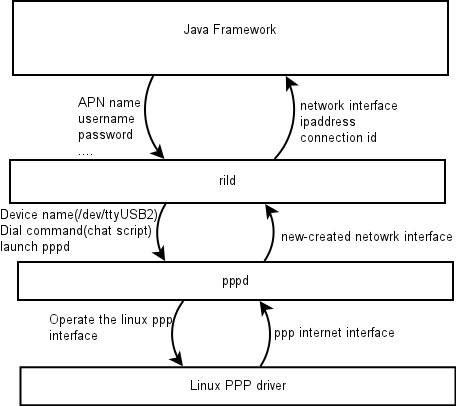
\includegraphics[height=2.5in]{ril/dataconn}}
\end{frame}

\begin{frame}
    \frametitle{CDMA Data conn Establish}
    \framebox{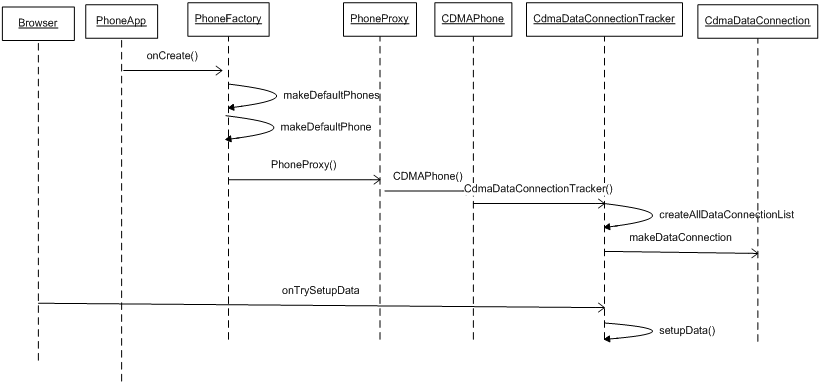
\includegraphics[height=2.5in]{ril/cdmadataconn}}
\end{frame}

\begin{frame}
    \frametitle{GSM Data conn Establish}
    \framebox{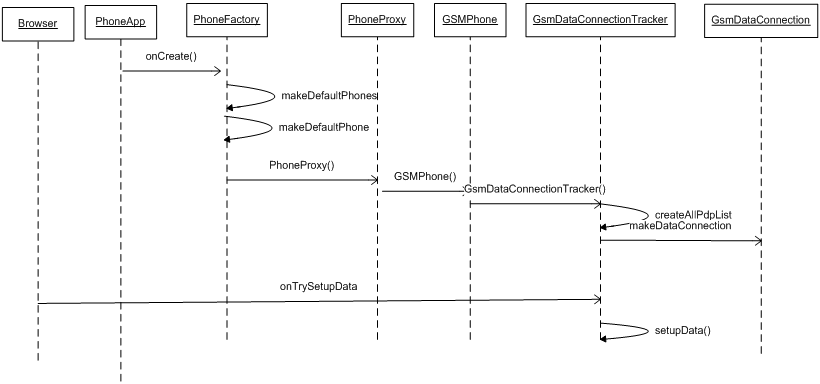
\includegraphics[height=2.5in]{ril/gsmdataconn}}
\end{frame}

\begin{frame}
    \frametitle{NOTES}
    \begin{itemize}
        \item A modem always have two channel to operate, when established a ppp link, one channel will be hold for ppp.
        \item pppd will create interface, set dns/ip or dhcp them.
    \end{itemize}
\end{frame}

\section{Reference}
\begin{frame}
    \frametitle{Reference}
    \begin{itemize}
        \item \href{http://www.netmite.com/android/mydroid/development/pdk/docs/telephony.html}{An Android Website}
        \item \href{http://www.slideshare.net/dpsmarques/android-ril}{Android RIL on SlideShare}
        \item \href{http://blogold.chinaunix.net/u3/93670/showart_2238540.html}{Androi RIL on EVDO/CDMA}
    \end{itemize}
\end{frame}

\end{document}

% vim:set fenc=utf8:
% vim:set ft=tex:


